\documentclass[a4paper]{article}

\usepackage[a4paper,margin=2cm]{geometry}
\usepackage{amsmath}
\usepackage{graphicx}
\usepackage[table]{xcolor}
\usepackage{tikz}
\usepackage{minted}
\usepackage[clock]{ifsym}
\usepackage{subcaption} % subfigures
\usepackage{hyperref} % links in table of contents
\usepackage[strings]{underscore}
\usepackage[sorting=none]{biblatex}

\usetikzlibrary{calc,positioning,arrows.meta,decorations.pathreplacing}
\graphicspath{ {./graphics/} }

\hypersetup{
	colorlinks,
	citecolor=black,
	filecolor=black,
	linkcolor=black,
	urlcolor=black
}
\numberwithin{figure}{section}
\numberwithin{table}{section}
\renewcommand{\arraystretch}{1.5}

\newcommand{\mi}{\mintinline}
\newcommand{\NA}{---}

\title{CS2031 - Assignment 1\\MQTT}
\date{2018-12-15}
\author{\url{https://git.nul.ie/dev/pubsub}\\\url{https://github.com/devplayer0/pubsub}\\Jack O'Sullivan\\\href{mailto:osullj19@tcd.ie}{osullj19@tcd.ie}}
\bibliography{bibliography}

\begin{document}
\maketitle
\tableofcontents
\pagenumbering{gobble}

\newpage
\pagenumbering{arabic}
\section{Introduction}
\subsection{Objective}
The goal of this assignment was to develop an implementation of an MQTT-like protocol making use of some kind of Flow Control.

Classic MQTT is implemented with TCP, which means it is guaranteed to deliver messages (in order). However, this can pose issues for embedded devices with limited resources, since TCP has some non-trivial overhead. Considering that MQTT publishers are often simple, low-power sensors - this problem is amplified.
For example, the ESP8266, a popular low-cost WiFi-enabled microcontroller \cite{esp8266} has a very small amount of memory (reduced even more once firmware is loaded \cite{esp8266-lowmem}).

\medskip
By designing a custom protocol with simple flow control (to ensure at least some degree of reliability), it should be more suitable for low-power devices. UDP, which is a relatively thin layer on top of a network-layer protocol like IPv4 or IPv6 (adding only source and destination port numbers along with a checksum) should be suitable.

\subsection{Flow control and error control}
In order to build a reliable communication channel on top of UDP, some kind of flow control is required. Flow control essentially places a limit on the amount of data that be sent before the receiver acknowledges receipt of the data. Some kind of error control is also usually employed to manage out-of-order or dropped packets.

For the purposes of this report, Selective-Repeat ARQ will not be discussed since it was not implemented by the solution for this assignment.

\subsubsection{Communication without flow control}
To understand the need for flow control and error control, it helps to examine the problems encountered when not using any.
\begin{figure}[h!]
	\centering
	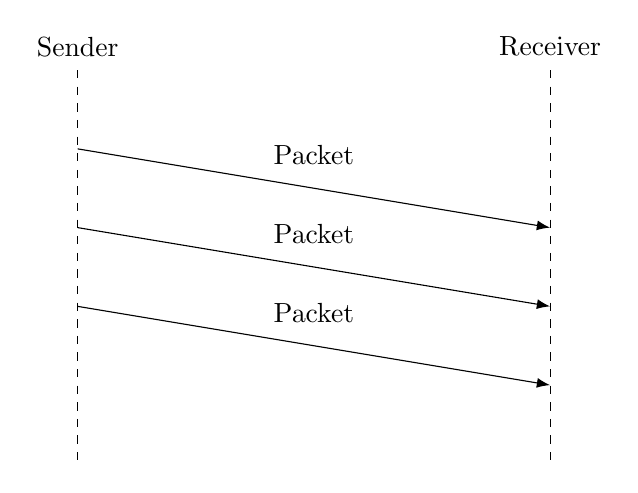
\begin{tikzpicture}
		\draw[dashed] (-3,0) -- (-3,-5) (3,0) -- (3,-5);
		\node at (-3,.3) {Sender};
		\node at (3,.3) {Receiver};

		\draw[-Latex] (-3,-1) -- node[midway,above=.5em] {Packet} (3,-2);
		\draw[-Latex] (-3,-2) -- node[midway,above=.5em] {Packet} (3,-3);
		\draw[-Latex] (-3,-3) -- node[midway,above=.5em] {Packet} (3,-4);
	\end{tikzpicture}
	\caption{No flow control: normal scenario}
	\label{fig:noflow-ok}
\end{figure}

\newpage
In Figure~\ref{fig:noflow-ok}, packets are delivered in order without any form of flow control, so clearly some form of communication is possible. However, as soon as any kind of errors appear (such as lost packets or out of order delivery), this quickly falls apart:

\begin{figure}[h!]
	\centering
	\begin{subfigure}[b][6cm][s]{.45\textwidth}
		\centering
		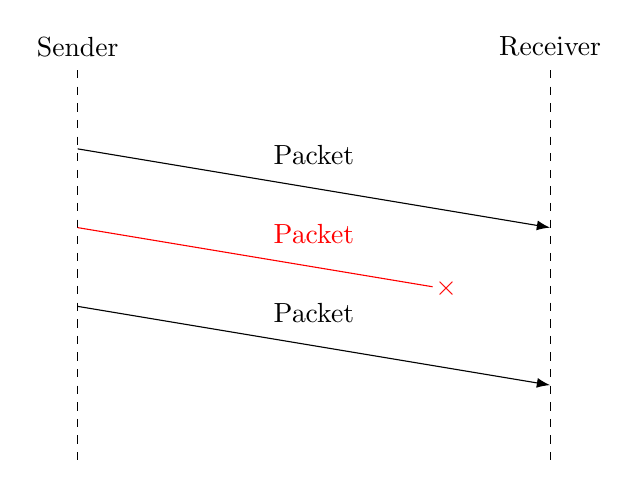
\begin{tikzpicture}
			\draw[dashed] (-3,0) -- (-3,-5) (3,0) -- (3,-5);
			\node at (-3,.3) {Sender};
			\node at (3,.3) {Receiver};

			\draw[-Latex] (-3,-1) -- node[midway,above=.5em] {Packet} (3,-2);
			\draw[color=red, dash pattern=on 130pt off 99pt] (-3,-2) -- node[midway,above=.5em] {Packet} (3,-3);
			\node[color=red] at ($(-3,-2)!135pt!(3,-3)$) {$\times$};

			\draw[-Latex] (-3,-3) -- node[midway,above=.5em] {Packet} (3,-4);
		\end{tikzpicture}
		\caption{Lost packet}
		\label{fig:noflow-lost}
	\end{subfigure}
	\begin{subfigure}[b][6cm][s]{.45\textwidth}
		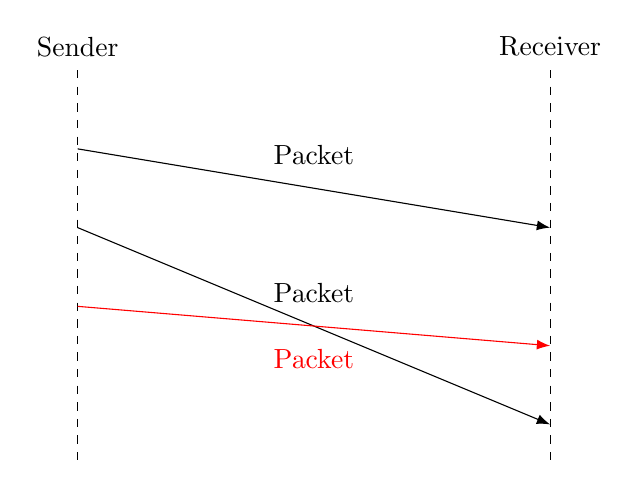
\begin{tikzpicture}
			\draw[dashed] (-3,0) -- (-3,-5) (3,0) -- (3,-5);
			\node at (-3,.3) {Sender};
			\node at (3,.3) {Receiver};

			\draw[-Latex] (-3,-1) -- node[midway,above=.5em] {Packet} (3,-2);
			\draw[-Latex] (-3,-2) -- node[midway,above=.5em] {Packet} (3,-4.5);
			\draw[-Latex, color=red] (-3,-3) -- node[midway,below=.5em] {Packet} (3,-3.5);
		\end{tikzpicture}
		\caption{Out of order delivery}
		\label{fig:noflow-ood}
	\end{subfigure}
	\caption{No flow control: error scenarios}
	\label{fig:noflow-errors}
\end{figure}

Figure~\ref{fig:noflow-lost} shows the second packet being dropped on its way to the receiver. There are a number of reasons that this could have happened (eg. packet contents too large for MTU). Regardless, the receiver will lose the data in the second packet completely and accept the third in its place. The receiver will always be 1 packet behind!

In Figure~\ref{fig:noflow-ood}, all of the packets are still delivered, but the third packet arrives before the second. Any switch / router between the sender and receiver could have caused the re-ordering for any reason, but since there is no way for the receiver to tell that it has received the third packet before the second, it will just accept the (most likely) invalid data in place of both the second and third packets.

\subsubsection{Stop-and-Wait}
Essentially the most simple form of flow control, Stop-and-Wait adds a an ACK (or acknowledgement) packet that the receiver must send in response to every sender packet \textbf{before the sender can continue}.
\begin{figure}[h!]
	\centering
	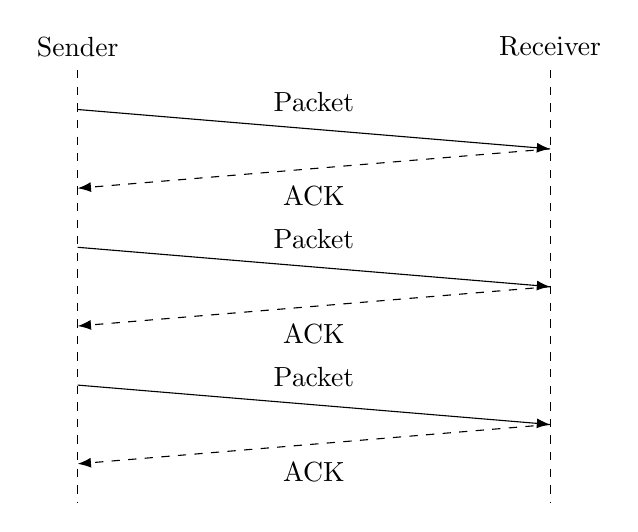
\begin{tikzpicture}
		\draw[dashed] (-3,0) -- (-3,-5.5) (3,0) -- (3,-5.5);
		\node at (-3,.3) {Sender};
		\node at (3,.3) {Receiver};

		\draw[-Latex] (-3,-.5) -- node[midway,above=.3em] {Packet} (3,-1);
		\draw[-Latex, dashed] (3,-1) -- node[midway,below=.3em] {ACK} (-3,-1.5);

		\draw[-Latex] (-3,-2.25) -- node[midway,above=.3em] {Packet} (3,-2.75);
		\draw[-Latex, dashed] (3,-2.75) -- node[midway,below=.3em] {ACK} (-3,-3.25);

		\draw[-Latex] (-3,-4) -- node[midway,above=.3em] {Packet} (3,-4.5);
		\draw[-Latex, dashed] (3,-4.5) -- node[midway,below=.3em] {ACK} (-3,-5);
	\end{tikzpicture}
	\caption{Stop-and-Wait}
	\label{fig:saw-ok}
\end{figure}

This is \textbf{flow control}: the sender can't push data down the pipe faster than the receiver can read it because it needs to wait for the ACK. Stop-and-Wait is \textit{not} error control, however:
\begin{itemize}
	\item In the case of lost packets (data or ACK), the sender will hang waiting for the client forever (to send an ACK for an unreceived packet or to re-send a dropped ACK) [Figure~\ref{fig:noflow-lost}]
	\item For packets delivered out of order, the receiver still can't tell that it has received incorrect data [Figure~\ref{fig:noflow-ood}]
\end{itemize}

\newpage
\subsubsection{Stop-and-Wait ARQ}
Stop-and-Wait ARQ (automatic repeat request) adds error control to Stop-and-Wait in order to solve the error scenarios in Figure~\ref{fig:noflow-errors}. This comes in the form of:
\begin{itemize}
	\item A 1-bit ``sequence number'' for packets and corresponding ACK's
	\item Sender timeouts: if an appropriate ACK is not received within a certain amount of time, re-send the last packet
\end{itemize}

\begin{figure}[h!]
	\centering
	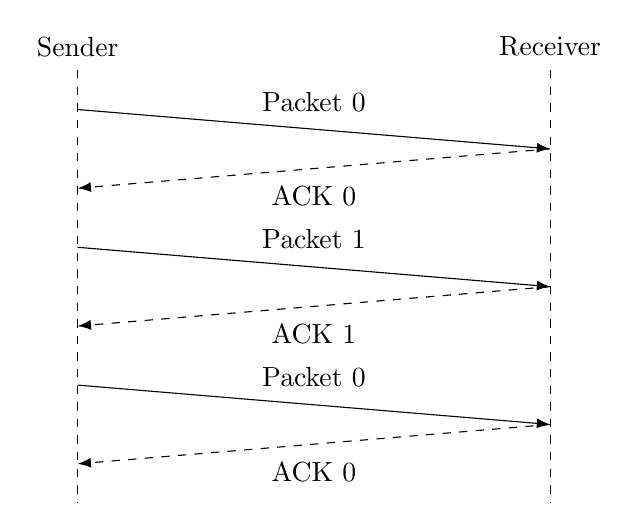
\begin{tikzpicture}
		\draw[dashed] (-3,0) -- (-3,-5.5) (3,0) -- (3,-5.5);
		\node at (-3,.3) {Sender};
		\node at (3,.3) {Receiver};

		\draw[-Latex] (-3,-.5) -- node[midway,above=.3em] {Packet 0} (3,-1);
		\draw[-Latex, dashed] (3,-1) -- node[midway,below=.3em] {ACK 0} (-3,-1.5);

		\draw[-Latex] (-3,-2.25) -- node[midway,above=.3em] {Packet 1} (3,-2.75);
		\draw[-Latex, dashed] (3,-2.75) -- node[midway,below=.3em] {ACK 1} (-3,-3.25);

		\draw[-Latex] (-3,-4) -- node[midway,above=.3em] {Packet 0} (3,-4.5);
		\draw[-Latex, dashed] (3,-4.5) -- node[midway,below=.3em] {ACK 0} (-3,-5);
	\end{tikzpicture}
	\caption{Stop-and-Wait ARQ: normal scenario}
	\label{fig:sawe-ok}
\end{figure}

As can be seen in Figure~\ref{fig:sawe-ok}, Stop-and-Wait ARQ looks very similar to plain Stop-and-Wait (without errors). The sender still waits for an ACK from the receiver before sending another data packet. However, Stop-and-Wait ARQ allows for dropped packets (either data or ACK's) to be recovered from:
\begin{figure}[h!]
	\centering
	\begin{subfigure}[b][6.5cm][s]{.45\textwidth}
		\centering
		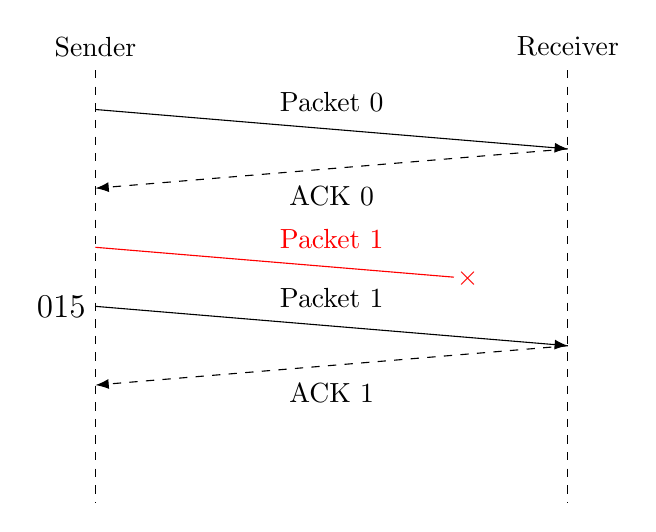
\begin{tikzpicture}
			\draw[dashed] (-3,0) -- (-3,-5.5) (3,0) -- (3,-5.5);
			\node at (-3,.3) {Sender};
			\node at (3,.3) {Receiver};

			\draw[-Latex] (-3,-.5) -- node[midway,above=.3em] {Packet 0} (3,-1);
			\draw[-Latex, dashed] (3,-1) -- node[midway,below=.3em] {ACK 0} (-3,-1.5);

			\draw[color=red, dash pattern=on 130pt off 99pt] (-3,-2.25) -- node[midway,above=.3em] {Packet 1} (3,-2.75);
			\node[color=red] at ($(-3,-2.25)!135pt!(3,-2.75)$) {$\times$};

			\node[anchor=east] at (-3,-3) {\large \showclock{0}{15}};
			\draw[-Latex] (-3,-3) -- node[midway,above=.3em] {Packet 1} (3,-3.5);
			\draw[-Latex, dashed] (3,-3.5) -- node[midway,below=.3em] {ACK 1} (-3,-4);
		\end{tikzpicture}
		\caption{Lost packet}
		\label{fig:sawe-lost}
	\end{subfigure}
	\begin{subfigure}[b][6.5cm][s]{.45\textwidth}
		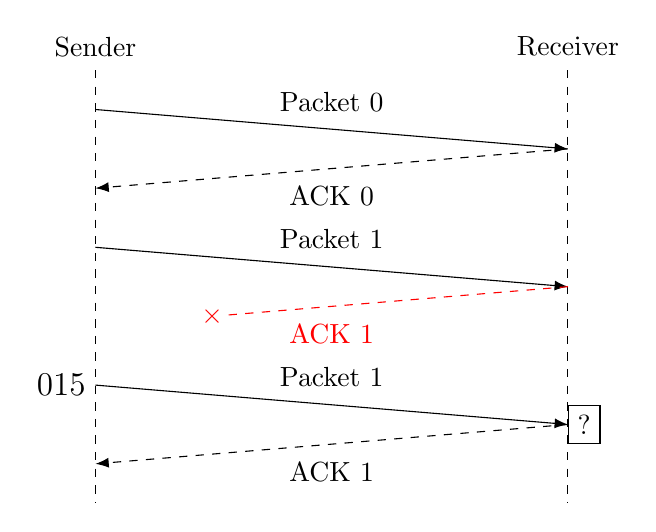
\begin{tikzpicture}
			\draw[dashed] (-3,0) -- (-3,-5.5) (3,0) -- (3,-5.5);
			\node at (-3,.3) {Sender};
			\node at (3,.3) {Receiver};

			\draw[-Latex] (-3,-.5) -- node[midway,above=.3em] {Packet 0} (3,-1);
			\draw[-Latex, dashed] (3,-1) -- node[midway,below=.3em] {ACK 0} (-3,-1.5);

			\draw[-Latex] (-3,-2.25) -- node[midway,above=.3em] {Packet 1} (3,-2.75);
			\draw[color=red, dash pattern=on 3pt off 3pt on 3pt off 3pt on 3pt off 3pt on 3pt off 3pt on 3pt off 3pt on 3pt off 3pt on 3pt off 3pt on 3pt off 3pt on 3pt off 3pt on 3pt off 3pt on 3pt off 3pt on 3pt off 3pt on 3pt off 3pt on 3pt off 3pt on 3pt off 3pt on 3pt off 3pt on 3pt off 3pt on 3pt off 3pt on 3pt off 3pt on 3pt off 3pt on 3pt off 99pt] (3,-2.75) -- node[midway,below=.3em] {ACK 1} (-3,-3.25);
			\node[color=red] at ($(3,-2.75)!129pt!(-3,-3.25)$) {$\times$};

			\node[anchor=east] at (-3,-4) {\large \showclock{0}{15}};
			\draw[-Latex] (-3,-4) -- node[midway,above=.3em] {Packet 1} (3,-4.5);
			\node[anchor=west, draw=black] at (3,-4.5) {?};

			\draw[-Latex, dashed] (3,-4.5) -- node[midway,below=.3em] {ACK 1} (-3,-5);
		\end{tikzpicture}
		\caption{Lost ACK}
		\label{fig:sawe-lack}
	\end{subfigure}
	\caption{Stop-and-Wait ARQ: dropped packet scenarios}
\end{figure}

Figure~\ref{fig:sawe-lost} shows Packet 1 never reaches the receiver. Since the receiver hasn't received Packet 1, it never sends an ACK. After a short time when the sender receives no ACK, it re-sends Packet 1 and upon receipt, the receiver sends an ACK and transmission continues.

In Figure~\ref{fig:sawe-lack}, Packet 1 reaches the receiver, but the corresponding ACK doesn't reach the sender. From the sender's perspective, this is the same situation as in Figure~\ref{fig:sawe-lost}, so it re-sends Packet 1 after a short timeout. This is when the 1-bit sequence number comes into play. When the receiver reads the re-transmitted Packet 1, it \textit{discards its contents} (because it has already seen this data - it knows this because of the sequence number) and sends another ACK.

\newpage
\subsubsection{Go-Back-N ARQ} \label{sec:gbn}
Although Stop-and-Wait ARQ can correct errors, it wastes bandwidth by allowing only a single data packet to be in-transit at once. Go-Back-N attempts to improve this through use of a sender ``sliding window''. Essentially, a sender can transmit up to $n$ packets (where $n$ is the window size) before needing to wait for the receiver to send an ACK.

\begin{figure}[h!]
	\centering
	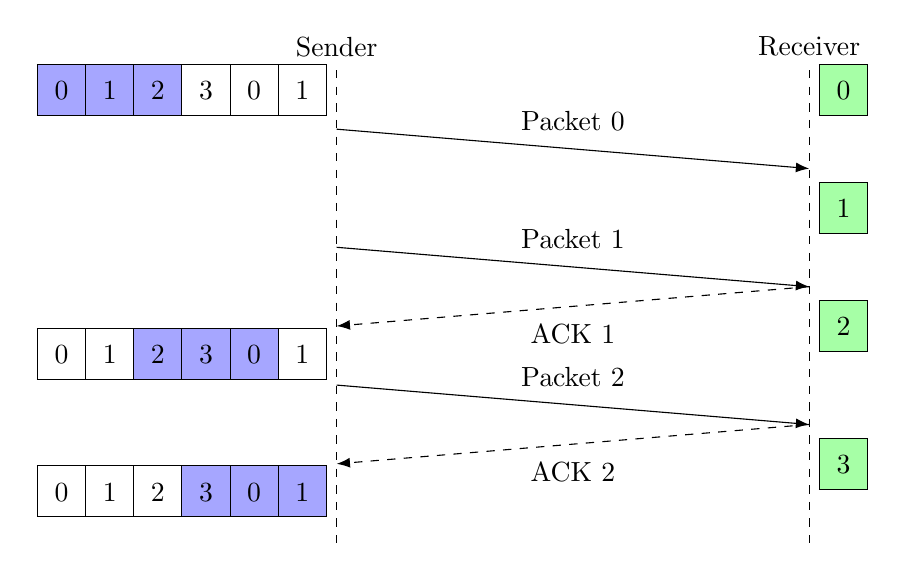
\begin{tikzpicture}
		\draw[dashed] (-3,0) -- (-3,-6) (3,0) -- (3,-6);
		\node at (-3,.3) {Sender};
		\node at (3,.3) {Receiver};

		\node[anchor=west] at (3,-.25) {\begin{tabular}{|c|}\hline \cellcolor{green!35}0 \\ \hline\end{tabular}};
		\node[anchor=west] at (3,-1.75) {\begin{tabular}{|c|}\hline \cellcolor{green!35}1 \\ \hline\end{tabular}};
		\node[anchor=west] at (3,-3.25) {\begin{tabular}{|c|}\hline \cellcolor{green!35}2 \\ \hline\end{tabular}};
		\node[anchor=west] at (3,-5) {\begin{tabular}{|c|}\hline \cellcolor{green!35}3 \\ \hline\end{tabular}};

		\draw[-Latex] (-3,-.75) -- node[midway,above=.3em] {Packet 0} (3,-1.25);

		\draw[-Latex] (-3,-2.25) -- node[midway,above=.3em] {Packet 1} (3,-2.75);
		\draw[-Latex, dashed] (3,-2.75) -- node[midway,below=.3em] {ACK 1} (-3,-3.25);

		\draw[-Latex] (-3,-4) -- node[midway,above=.3em] {Packet 2} (3,-4.5);
		\draw[-Latex, dashed] (3,-4.5) -- node[midway,below=.3em] {ACK 2} (-3,-5);

		\node[anchor=east] at (-3,-.25) {\begin{tabular}{|c|c|c|c|c|c|}\hline \cellcolor{blue!35}0&\cellcolor{blue!35}1&\cellcolor{blue!35}2&3&0&1 \\ \hline\end{tabular}};
		\node[anchor=east] at (-3,-3.6) {\begin{tabular}{|c|c|c|c|c|c|}\hline 0&1&\cellcolor{blue!35}2&\cellcolor{blue!35}3&\cellcolor{blue!35}0&1 \\ \hline\end{tabular}};
		\node[anchor=east] at (-3,-5.35) {\begin{tabular}{|c|c|c|c|c|c|}\hline 0&1&2&\cellcolor{blue!35}3&\cellcolor{blue!35}0&\cellcolor{blue!35}1 \\ \hline\end{tabular}};
	\end{tikzpicture}
	\caption{Go-Back-N ARQ: normal scenario}
	\label{fig:gbn-ok}
\end{figure}

The blue shaded numbers in Figure~\ref{fig:gbn-ok} represent the current send window - when an ACK is received the window shifts forward past the number in the ACK packet. This means that not every packet \textit{has} to be acknowledged. Also of note is the fact that the size of the window is 1 less than the highest sequence number. This is important for handling errors. The window size can therefore be calculated as $2^m - 1$ where $m$ is the number of bits used for the sequence number.

The green shaded numbers on the right represent the receiver ``window''. This is the only sequence number packet that the receiver will accept at that point, others will be ignored. On receipt of a packet, this number is incremented (wrapping around of course) and an acknowledgement packet is usually sent.

\medskip
If data packets or ACK's are lost, after a short timeout the sender will re-send all of the packets in the current send window (similarly to Stop-and-Wait ARQ). The requirement for $w = 2^m - 1$ can be understood by looking at the following error scenario:
\begin{figure}[h!]
	\centering
	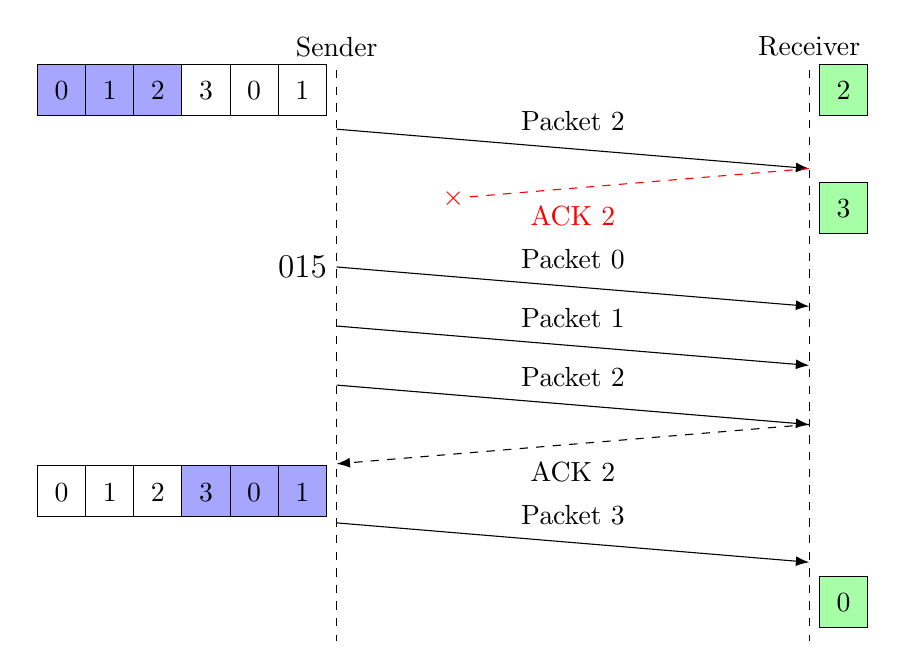
\begin{tikzpicture}
		\draw[dashed] (-3,0) -- (-3,-7.25) (3,0) -- (3,-7.25);
		\node at (-3,.3) {Sender};
		\node at (3,.3) {Receiver};

		\node[anchor=west] at (3,-.25) {\begin{tabular}{|c|}\hline \cellcolor{green!35}2 \\ \hline\end{tabular}};
		\node[anchor=west] at (3,-1.75) {\begin{tabular}{|c|}\hline \cellcolor{green!35}3 \\ \hline\end{tabular}};
		\node[anchor=west] at (3,-6.75) {\begin{tabular}{|c|}\hline \cellcolor{green!35}0 \\ \hline\end{tabular}};

		\draw[-Latex] (-3,-.75) -- node[midway,above=.3em] {Packet 2} (3,-1.25);
		\draw[color=red, dash pattern=on 3pt off 3pt on 3pt off 3pt on 3pt off 3pt on 3pt off 3pt on 3pt off 3pt on 3pt off 3pt on 3pt off 3pt on 3pt off 3pt on 3pt off 3pt on 3pt off 3pt on 3pt off 3pt on 3pt off 3pt on 3pt off 3pt on 3pt off 3pt on 3pt off 3pt on 3pt off 3pt on 3pt off 3pt on 3pt off 3pt on 3pt off 3pt on 3pt off 3pt on 3pt off 99pt] (3,-1.25) -- node[midway,below=.3em] {ACK 2} (-3,-1.75);
		\node[color=red] at ($(3,-1.25)!129pt!(-3,-1.75)$) {$\times$};

		\node[anchor=east] at (-3,-2.5) {\large \showclock{0}{15}};
		\draw[-Latex] (-3,-2.5) -- node[midway,above=.3em] {Packet 0} (3,-3);
		\draw[-Latex] (-3,-3.25) -- node[midway,above=.3em] {Packet 1} (3,-3.75);
		\draw[-Latex] (-3,-4) -- node[midway,above=.3em] {Packet 2} (3,-4.5);
		\draw[-Latex, dashed] (3,-4.5) -- node[midway,below=.3em] {ACK 2} (-3,-5);

		\draw[-Latex] (-3,-5.75) -- node[midway,above=.3em] {Packet 3} (3,-6.25);

		\node[anchor=east] at (-3,-.25) {\begin{tabular}{|c|c|c|c|c|c|}\hline \cellcolor{blue!35}0&\cellcolor{blue!35}1&\cellcolor{blue!35}2&3&0&1 \\ \hline\end{tabular}};
		\node[anchor=east] at (-3,-5.35) {\begin{tabular}{|c|c|c|c|c|c|}\hline 0&1&2&\cellcolor{blue!35}3&\cellcolor{blue!35}0&\cellcolor{blue!35}1 \\ \hline\end{tabular}};
	\end{tikzpicture}
	\caption{Go-Back-N ARQ: many ACK's lost}
	\label{fig:gbn-bad}
\end{figure}

\newpage
In Figure~\ref{fig:gbn-bad}, it can be assumed that the sender has sent packets 0 and 1 (with no ACK from the receiver) before this diagram starts.

When the sender fails to receive any acknowledgement, it re-sends all of the packets in the window as described above. The receiver's expected packet doesn't change since it has already received packets 0 to 2, but it sends an ACK at the end. Note that if the packets 0 through 3 had been sent without acknowledgement (and re-sent again after a timeout), the receiver would have wrapped around and \textbf{accept the the re-sent packets as new data}!

\section{Implementation}
The implementation of the assignment is called ``JQTT'' (Jack's Queueing Telemetry Transport).
\subsection{Design choices / features}
\begin{itemize}
	\item Rust was used as the main language for its high-level features combined with high performance \cite{rust-lang}
	\item The assignment was split into a number of subprojects:
		\begin{itemize}
			\item \mi{c}{pubsub-broker}: JQTT broker library
			\item \mi{c}{pubsub-client}: JQTT publisher / subscriber library
			\item \mi{c}{pubsub-common}: Common code used by broker / client
			\item \mi{c}{pubsub-server}: Command line application which starts a broker using the \mi{c}{pubsub-broker} library
			\item \mi{c}{pubsub-client}: Interactive client demo with publish / subscribe in an \mi{c}{ncurses}-like UI
			\item \mi{c}{pubsub-demos}: Additional mini command line demos
		\end{itemize}
	\item Go-Back-N was used as the flow control method of choice (with a window size of 15)
	\item Messages can (in theory) be up to 4GB (32-bit) in size thanks to multi-packet messages
	\item More than one multi-packet message can be in-flight at a time
	\item A Wireshark dissector was written for the wire protocol to make debugging easier
\end{itemize}

\subsection{Protocol} \label{sec:protocol}
The JQTT protocol is made up of 9 different packet types. Each is made up of a 1 byte header and (usually) some kind of payload. All integers are in network / big endian. The header looks like this:

\newcommand*{\tn}[2]{\tikz[baseline,remember picture]\node[inner sep=0pt,outer sep=2pt,anchor=base] (#1) {#2};}
\begin{figure}[h!]
	\centering
	\begin{tabular}{|c|c|c|c|c|c|c|c|}
		\hline
		\cellcolor{red!30}\tn{type-start}{0} &\cellcolor{red!30}0&\cellcolor{red!30}1& \cellcolor{red!30}\tn{type-end}{1} & \cellcolor{blue!30}\tn{seq-start}{0} &\cellcolor{blue!30}1&\cellcolor{blue!30}0& \cellcolor{blue!30}\tn{seq-end}{0} \\
		\hline
	\end{tabular}

	\begin{tikzpicture}[remember picture, overlay]
		\draw[decorate, decoration={brace,amplitude=5pt,mirror,raise=5pt}] (type-start.south west) -- (type-end.south east) node[midway, below=10pt] {Type (\mi{c}{ACK})};
		\draw[decorate, decoration={brace,amplitude=5pt,mirror,raise=5pt}] (seq-start.south west) -- (seq-end.south east) node[midway, below=10pt] {Sequence no. (\mi{c}{4})};
	\end{tikzpicture}
	\vspace*{10pt}
	\caption{Header layout}
	\label{fig:packet-header}
\end{figure}

Figure~\ref{fig:packet-header} shows the first four bits of the header represent the packet type (in the range \mi{c}{0} to \mi{c}{8} inclusive).

The last 4 bits represent the sequence number of the packet, if relevant. In this example, the packet is an acknowledgement for the packet with sequence number 4. For unordered packets (such as \mi{c}{HEARTBEAT}), the contents of these bits is irrelevant.

\newpage
\subsubsection{Wireshark dissector}
The Wireshark dissector for this assignment was written in Lua (see \mi{c}{wireshark_dissector.lua}). Drop it into the plugin folder of your local Wireshark installation (\mi{c}{~/.local/lib/wireshark/plugins} on Linux) to install it. When enabled, JQTT packets will be decoded:

\begin{figure}[h!]
	\centering
	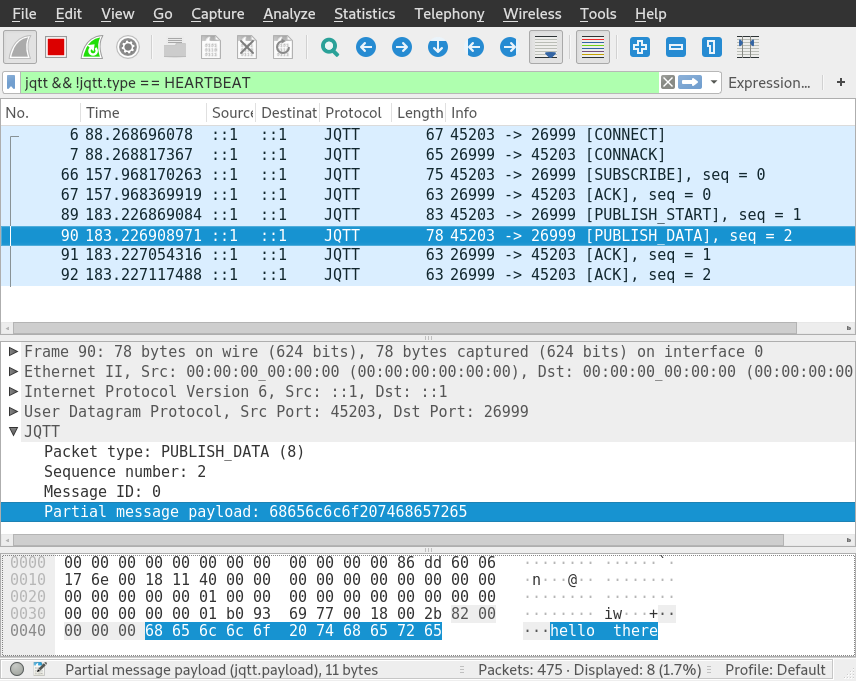
\includegraphics[width=\textwidth]{dissector}
	\caption{JQTT packets decoded in Wireshark}
	\label{fig:dissector}
\end{figure}

Figure~\ref{fig:dissector} shows JQTT packets decoded from raw UDP with detailed output. The filter field can be used to show only certain packets based on field values. In this example, \mi{c}{jqtt && !jqtt.type == HEARTBEAT} will show only JQTT packets that aren't of the \mi{c}{HEARTBEAT} type. Clicking on the 'Expression\dots' button and expanding the 'JQTT' tree will show possible field names and a brief explanation.

The 'Info' column shows the source and destination port numbers, the packet type (in square brackets) and the sequence number (if applicable).

Selecting a packet and expanding the JQTT section will show the packet type, sequence number as well as any packet-specific payload information. Clicking on a field will highlight the portion of the hex dump view its contents represents.

\newpage
\subsection{Packet types}
As explained in section~\ref{sec:protocol}, there are 9 distinct pacet types in JQTT. The structure and purpose of each is explained in detail in this section (in order of the type number given to each; \mi{c}{CONNECT} is \mi{c}{0}, \mi{c}{CONNACK} is \mi{c}{1} etc.).

\subsubsection{\mi{c}{CONNECT}}
The \mi{c}{CONNECT} packet is sent by any client (publisher / subscriber or both) to establish a ``connection'' state with a broker. The packet type is \mi{c}{0} and the sequence bits are unused. 4 magic bytes appear after the header in the form of the ASCII representation of the string ``JQTT''.

In response to this packet the broker will send a \mi{c}{CONNACK} packet. After this the server will no longer accept \mi{c}{CONNECT} packets from this client until it disconnects or times out (if \mi{c}{keepalive} is enabled). If the client fails to receive a \mi{c}{CONNACK} response within a certain time, it will send another \mi{c}{CONNECT} packet (up to 5 times).

\subsubsection{\mi{c}{CONNACK}}
Upon receiving a \mi{c}{CONNECT} packet from a client, the broker will send a \mi{c}{CONNACK} packet in reponse (as described above). It contains:
\begin{itemize}
	\item A flags bitfield (in place of the sequence number bits) - currently the only flag (the lowest bit) is whether the broker has \mi{c}{keepalive} mode enabled (see section~\ref{sec:heartbeat} on the \mi{c}{HEARTBEAT} packet)
	\item A 16-bit unsigned integer representing the maximum packet size (including the 1 byte header) - this affects the packet types with variable length payloads
\end{itemize}

\subsubsection{\mi{c}{HEARTBEAT}} \label{sec:heartbeat}
Under \mi{c}{keepalive} mode, clients must send a \mi{c}{HEARTBEAT} packet to the broker every few seconds. The server will respond to each \mi{c}{HEARTBEAT} packet with its own. If either the server or the client has not received a \mi{c}{HEARTBEAT} packet within the last 5 seconds, it will consider the peer as ``timed out'' and ``disconnect'' it (sending a \mi{c}{DISCONNECT} packet).

In terms of structure, \mi{c}{HEARTBEAT} is very simple. It contains only the 1-byte JQTT header with all of the sequence bits set to 0 since it is not packet which needs to be delivered in the correct order (or at all, since it contains no information and another will take its place if lost).

\subsubsection{\mi{c}{ACK}}
The \mi{c}{ACK} packet simply fills the acknowledgement packet role required for Go-Back-N (as described in section~\ref{sec:gbn}). It is sent by both clients and the broker for all ordered packets.

Like \mi{c}{HEARTBEAT}, \mi{c}{ACK} is consists of only the 1-byte header. The sequence bits represent the sequence number of the packet being acknowledged.

\subsubsection{\mi{c}{DISCONNECT}}
\mi{c}{DISCONNECT} can be sent to either clients or a broker to indicate that the ``connection'' between the two should be stopped. It can be sent for a variety of reasons:
\begin{itemize}
	\item A client is terminating and informs the server
	\item The broker is terminating and is informing all clients
	\item A client / broker timed out in \mi{c}{keepalive} mode
	\item A malformed / invalid packet was received by a client or broker
	\item There was an error sending a packet (e.g. operating system related)
\end{itemize}

This is another header-only packet. The sequence bits are used since \mi{c}{DISCONNECT} needs to be delivered reliably.

\subsubsection{\mi{c}{SUBSCRIBE}}
When a client wishes to subscribe to messages published to a topic, it sends a \mi{c}{SUBSCRIBE} packet. The broker will add the client to the list of subscribers for that topic and dispatch any messages that arrive \textit{after} subscribing (the broker will not dispatch messages to a subscriber that were published to a topic prior to subscription).

\medskip
\mi{c}{SUBSCRIBE} obviously makes use of the sequence bits since it should be delivered reliably. After the header, the remainder of the packet is a UTF-8 encoded string (\textbf{not} null-terminated). Since a UDP packet has a distinct size, the length of the string can be determined by subtracting 1 (for the header) from the UDP payload size.

\medskip
Note that the maximum packet length (as provided by the broker to clients in the \mi{c}{CONNACK} packet) determines the longest possible topic length! See section~\ref{sec:pubstart} for an explanation on how the maximum length of a topic string is calculated.

\subsubsection{\mi{c}{UNSUBSCRIBE}}
The \mi{c}{UNSUBSCRIBE} packet is very simple. When a broker receives this packet it will remove the client from the list of subscribers for that topic. The client will no longer receive any messages published to that topic. Its structure is identical to that of \mi{c}{SUBSCRIBE}.

\subsubsection{\mi{c}{PUBLISH_START}} \label{sec:pubstart}
This is one of the most important packets. \mi{c}{PUBLISH_START} contains information about a message which is about to me published in one or more \mi{c}{PUBLISH_DATA} packets. It can be sent by both clients \textit{and} brokers depending on the context:
\begin{itemize}
	\item Clients send this packet when they wish to publish a message to a topic
	\item A broker will send this packet to all subscribers of a topic upon receiving a \mi{c}{PUBLISH_START} packet from a client (\textbf{with the exception of the publisher of the message})
\end{itemize}

\mi{c}{PUBLISH_START} contains 3 fields, they are (in order of appearance in the packet):
\begin{itemize}
	\item Message ID: A 32-bit unsigned integer which allows multiple messages to be ``in-flight'' simultaneously. Since message data is split across a multitude of \mi{c}{PUBLISH_DATA} packets, this is very useful (especially if a large message is in the process of being sent). Also of note is the fact that this ID is different based on who sent the packet. If it was sent by a client (asking a broker to publish a message to subscribers), it is unique to that client only. When a server is dispatching the \mi{c}{PUBLISH_START} to subscribers, it will overwrite the message ID with a value unique across all subscribers of all topics the broker holds.
	\item Message size: Another 32-bit unsigned integer which indicates the size (in bytes) of the message payload (to be split across a number of \mi{c}{PUBLISH_DATA} packets)
	\item Topic: This is a UTF-8 encoded string indicating the topic to which this message should be published. As with \mi{c}{SUBSCRIBE} and \mi{c}{UNSUBSCRIBE}, the length of this string is determined by the remaining bytes in the UDP payload. \textbf{The largest possible topic is determined by this packet - this applies to \mi{c}{SUBSCRIBE} and \mi{c}{UNSUBSCRIBE} too since a topic name could conceivably fit into these smaller packets but \underline{not} in a \mi{c}{PUBLISH_START} packet.}
\end{itemize}

\subsubsection{\mi{c}{PUBLISH_DATA}}
Where \mi{c}{PUBLISH_START} starts the publishing process for a message, \mi{c}{PUBLISH_DATA} contains (at least some of) the actual message payload.

Like \mi{c}{PUBLISH_START}, it can be sent by either the client (if that client is the one publishing the message) or a broker (distributing the message to subscribers on behalf of the publisher). This packet consists of two fields:
\begin{itemize}
	\item Message ID: A 32-bit unsigned integer which must match that of a preceding \mi{c}{PUBLISH_START} packet - if a data packet is sent without a start packet, the receiver will complain. The same applies if a data packet is sent and the total transmitted data for that message ID would exceed the value set in the initial \mi{c}{PUBLISH_START} packet.
	\item Actual (partial) message payload: The remainder of the packet is data \textbf{of an arbitrary format}. A publisher will split the full payload into a number of \mi{c}{PUBLISH_DATA} packets based on the maximum packet size set out in the \mi{c}{CONNACK} packet for the connection. When subscribers receive the published packets from a broker they will re-assemble the segments into the original payload.
\end{itemize}

\clearpage
\phantomsection
\addcontentsline{toc}{section}{References}
\printbibliography

\end{document}
# vim: nofoldenable
